% 1988 年广东卷文史类第一卷第 24 小题：固定源中的折线图
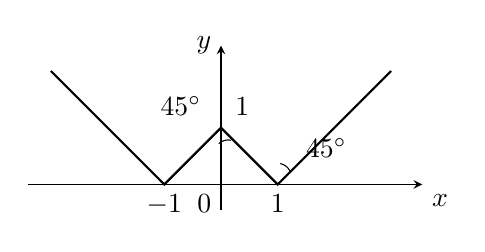
\begin{tikzpicture}[scale=0.72,>=stealth]
  \draw[->] (-3.4,0)--(3.55,0) node[below right] {$x$};
  \draw[->] (0,-0.45)--(0,2.45) node[left] {$y$};
  \draw[thick] (-3.0,2)--(-1,0)--(0,1)--(1,0)--(3.0,2);
  \draw (0.18,0.78) arc (78:132:0.25);
  \draw (1.22,0.23) arc (25:78:0.25);
  \node[above right] at (0.08,1.05) {$1$};
  \node[below left] at (0,0) {$0$};
  \node[below] at (-1,0) {$-1$};
  \node[below] at (1,0) {$1$};
  \node[above left] at (-0.18,1.05) {$45^\circ$};
  \node[above right] at (1.33,0.30) {$45^\circ$};
\end{tikzpicture}
